\section{Prueba en hardware real (FPGA Basys 3)}

Finalmente, se validó la implementación sintetizada en la FPGA Basys 3. Se cargó el bitstream generado por Vivado y se ejecutaron pruebas controladas de operaciones aritméticas y lógicas, utilizando los switches como entradas y los botones para cargar operandos/operaciones. Los resultados se observaron en los LEDs y en el display de 7 segmentos integrado en la placa.

\subsection{Secuencia de pruebas}

\begin{enumerate}
    \item \textbf{Reset inicial:} tras aplicar \texttt{rst}, la placa muestra el estado limpio en el display (Figura~\ref{fig:fpga1}).

    \item \textbf{Carga de A = 10000:} se coloca el valor en los switches y se pulsa \texttt{btn\_a} (Figura~\ref{fig:fpga2}).

    \item \textbf{Suma con operandos cargados:} al cargar la operación de suma, se observa el resultado correcto en el display (Figuras~\ref{fig:fpga3} y \ref{fig:fpga4}).

    \item \textbf{Operación SRA con A = 11:} se carga el operando y la operación de corrimiento aritmético a derecha. El resultado en el display coincide con lo esperado (Figura~\ref{fig:fpga5}).

    \item \textbf{Variación de B:} se prueba con diferentes valores de B (1, 0 y 100), confirmando el funcionamiento de la ALU en cada caso (Figuras~\ref{fig:fpga6}, \ref{fig:fpga7} y \ref{fig:fpga8}).
\end{enumerate}

\subsection{Resultados}
En todos los casos, los resultados observados en LEDs y display coinciden con los valores esperados de acuerdo con la simulación previa, validando la correcta implementación del diseño.

\begin{figure}[H]
    \centering
    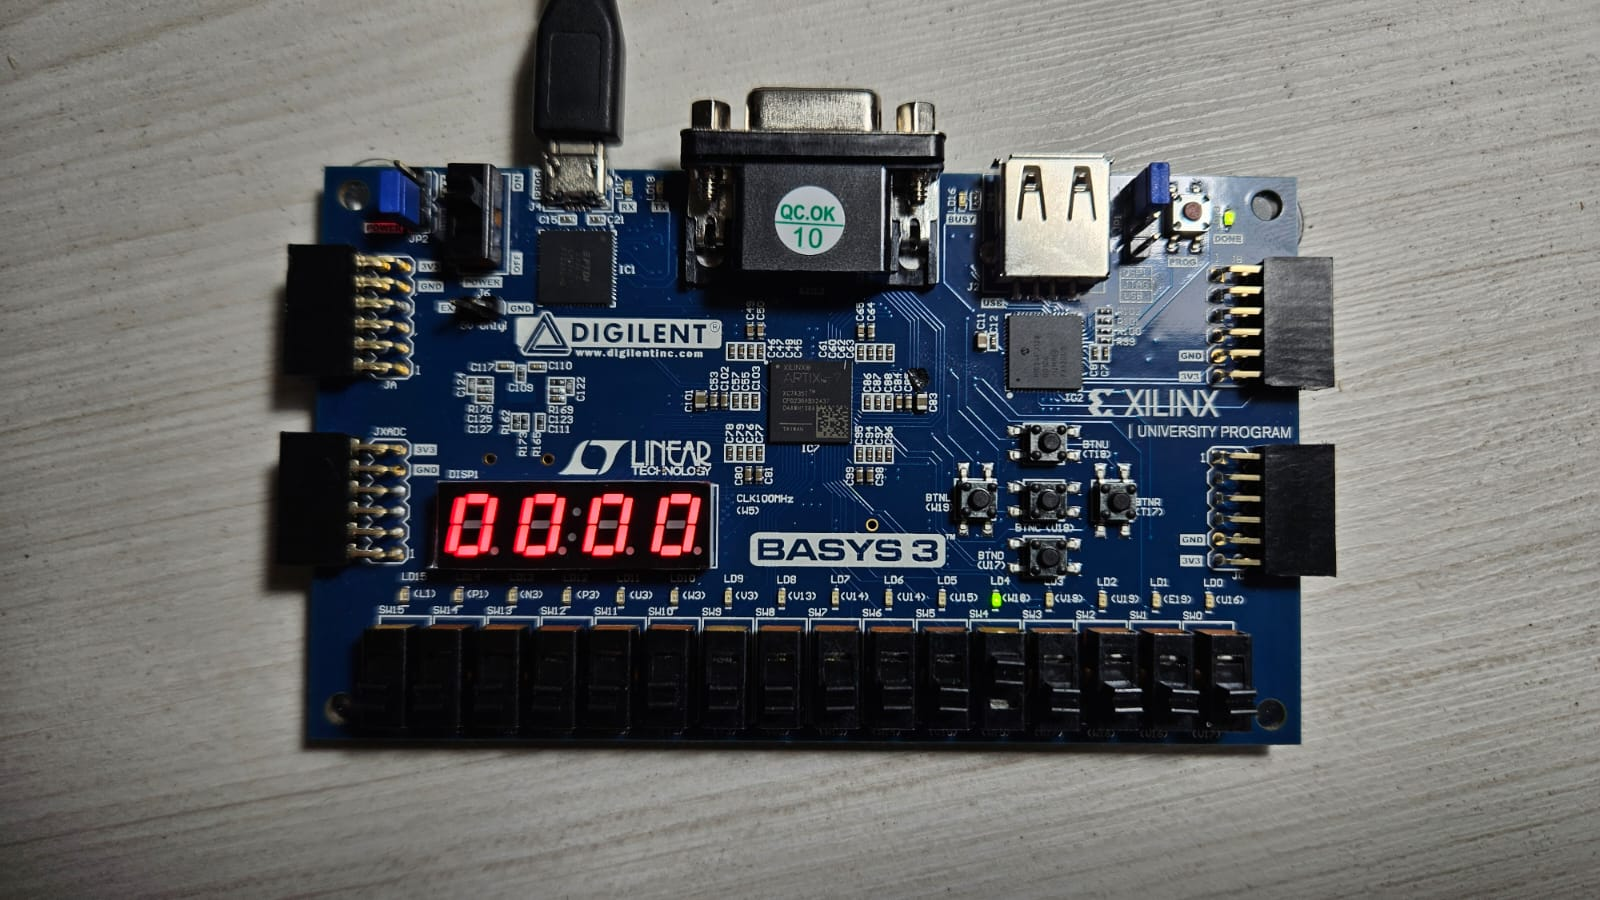
\includegraphics[width=0.6\textwidth]{img/fpga1.png}
    \caption{Carga de $A=10000$ después del \texttt{reset}.}
    \label{fig:fpga1}
\end{figure}

\begin{figure}[H]
    \centering
    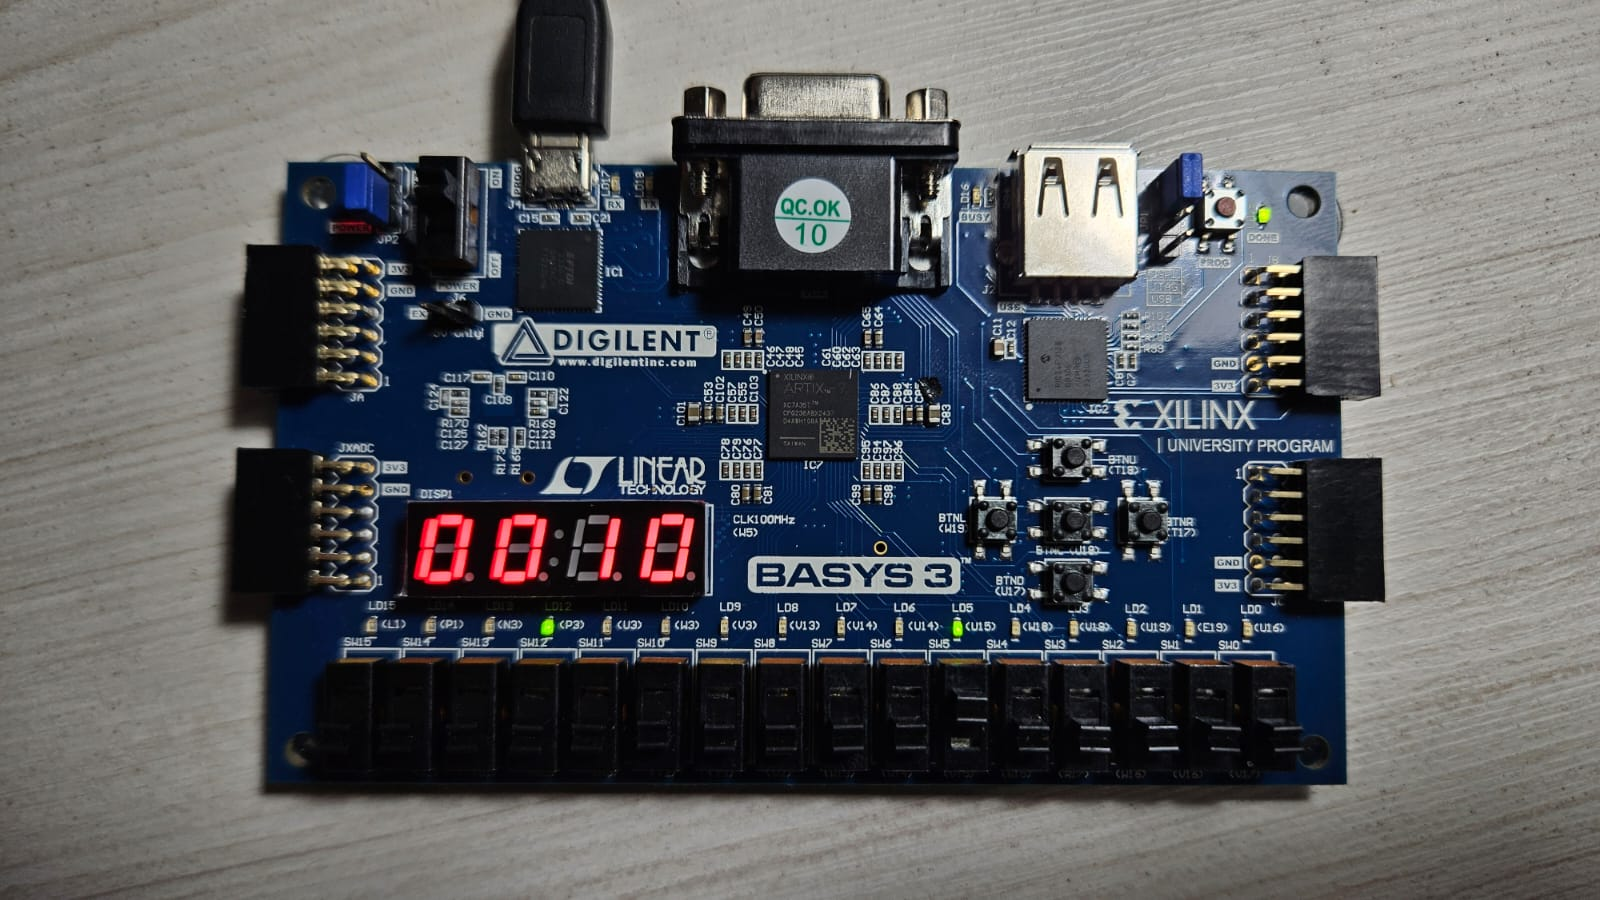
\includegraphics[width=0.6\textwidth]{img/fpga2.png}
    \caption{Carga de la suma después de cargar A.}
    \label{fig:fpga2}
\end{figure}

\begin{figure}[H]
    \centering
    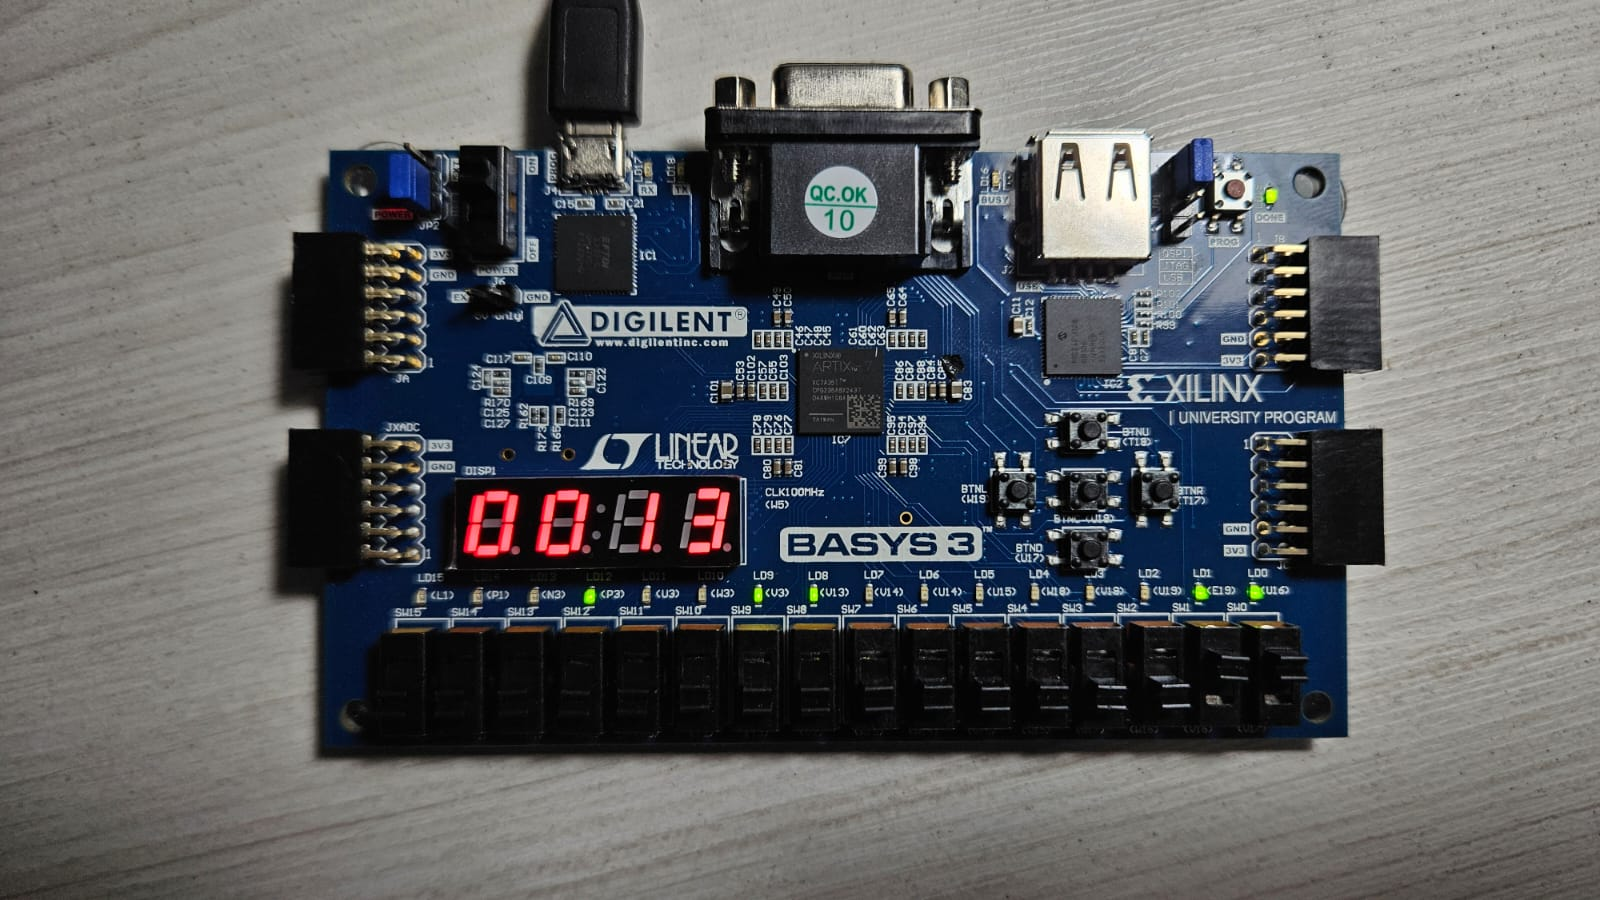
\includegraphics[width=0.6\textwidth]{img/fpga3.png}
    \caption{Carga de $B=11$, se observa el resultado de la suma ($10011$).}
    \label{fig:fpga3}
\end{figure}

\begin{figure}[H]
    \centering
    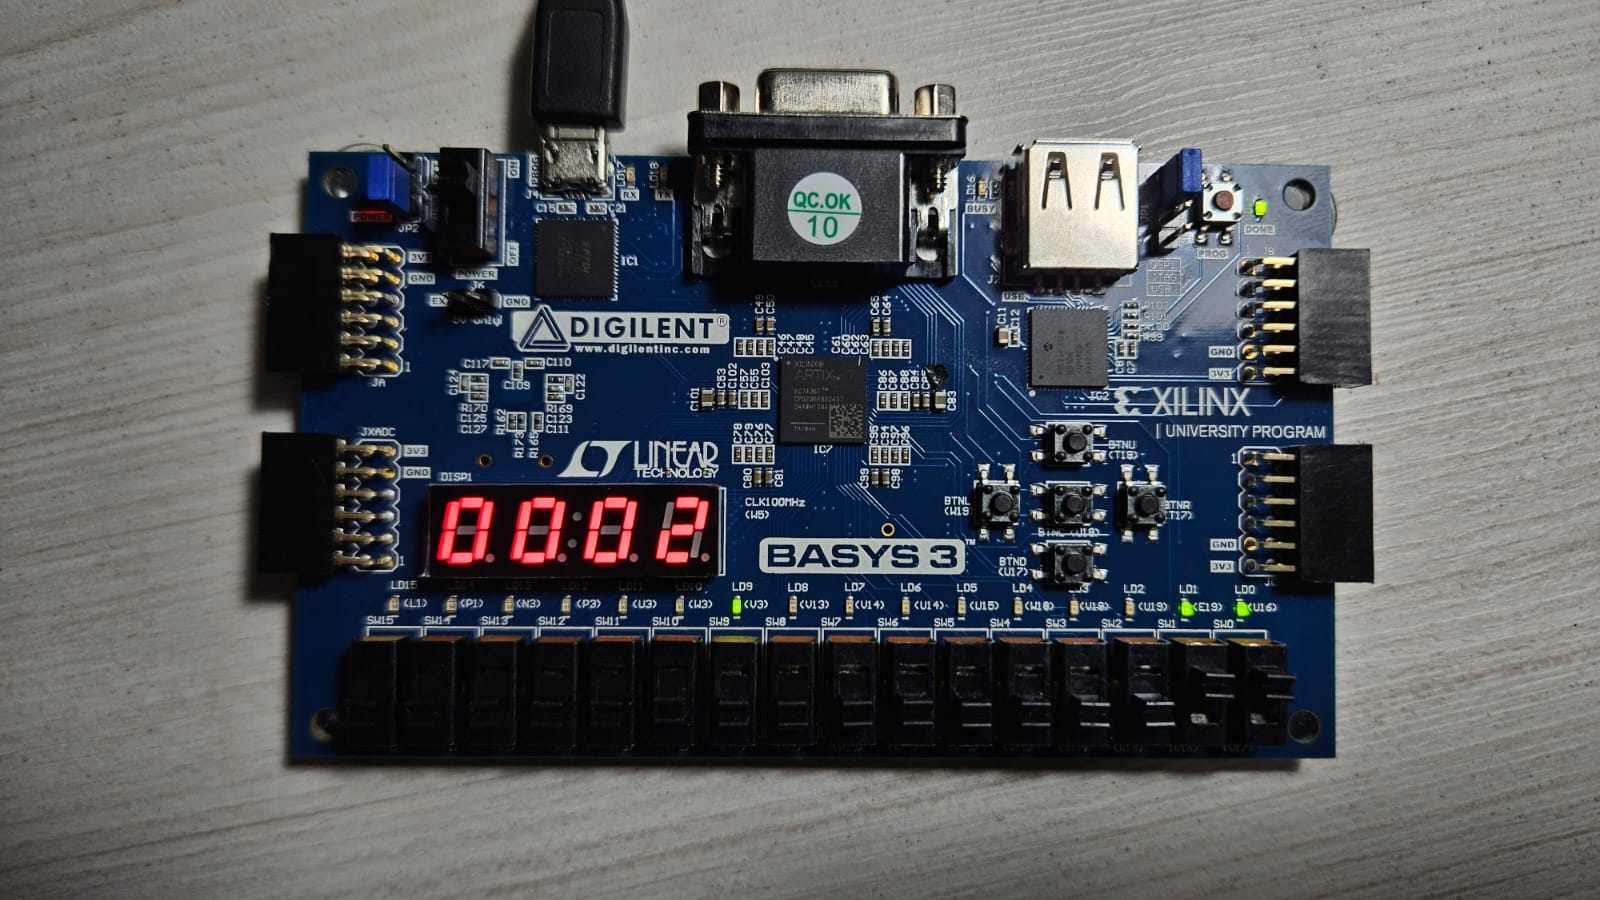
\includegraphics[width=0.6\textwidth]{img/fpga4.png}
    \caption{Carga de la operación SRA con $A=11$.}
    \label{fig:fpga4}
\end{figure}

\begin{figure}[H]
    \centering
    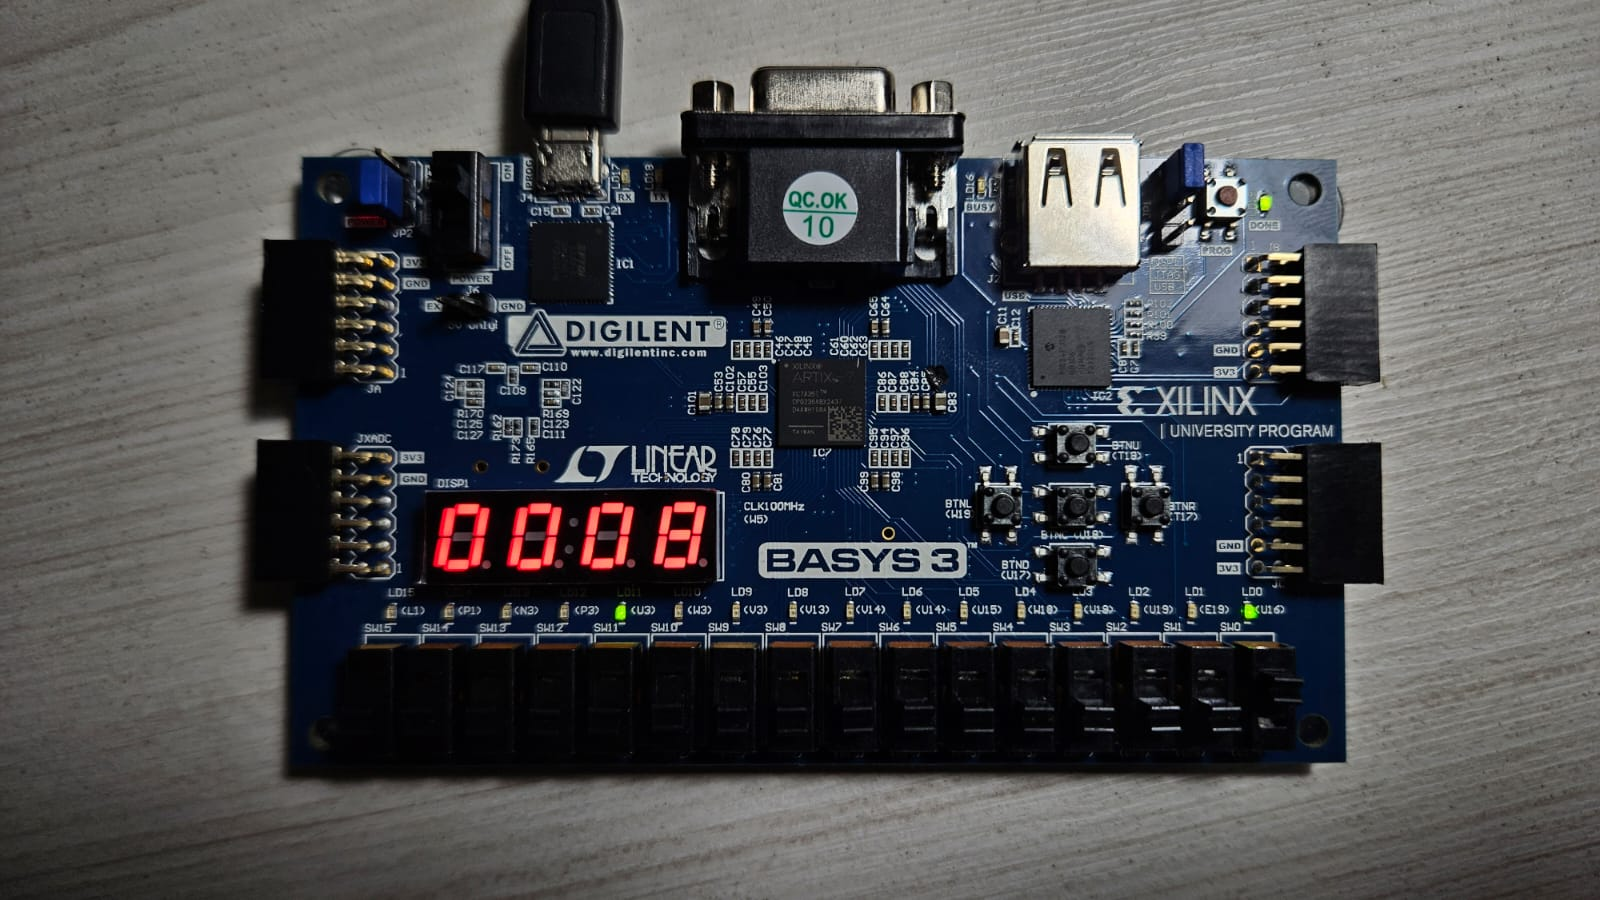
\includegraphics[width=0.6\textwidth]{img/fpga5.png}
    \caption{Prueba con $B=1$.}
    \label{fig:fpga5}
\end{figure}

\begin{figure}[H]
    \centering
    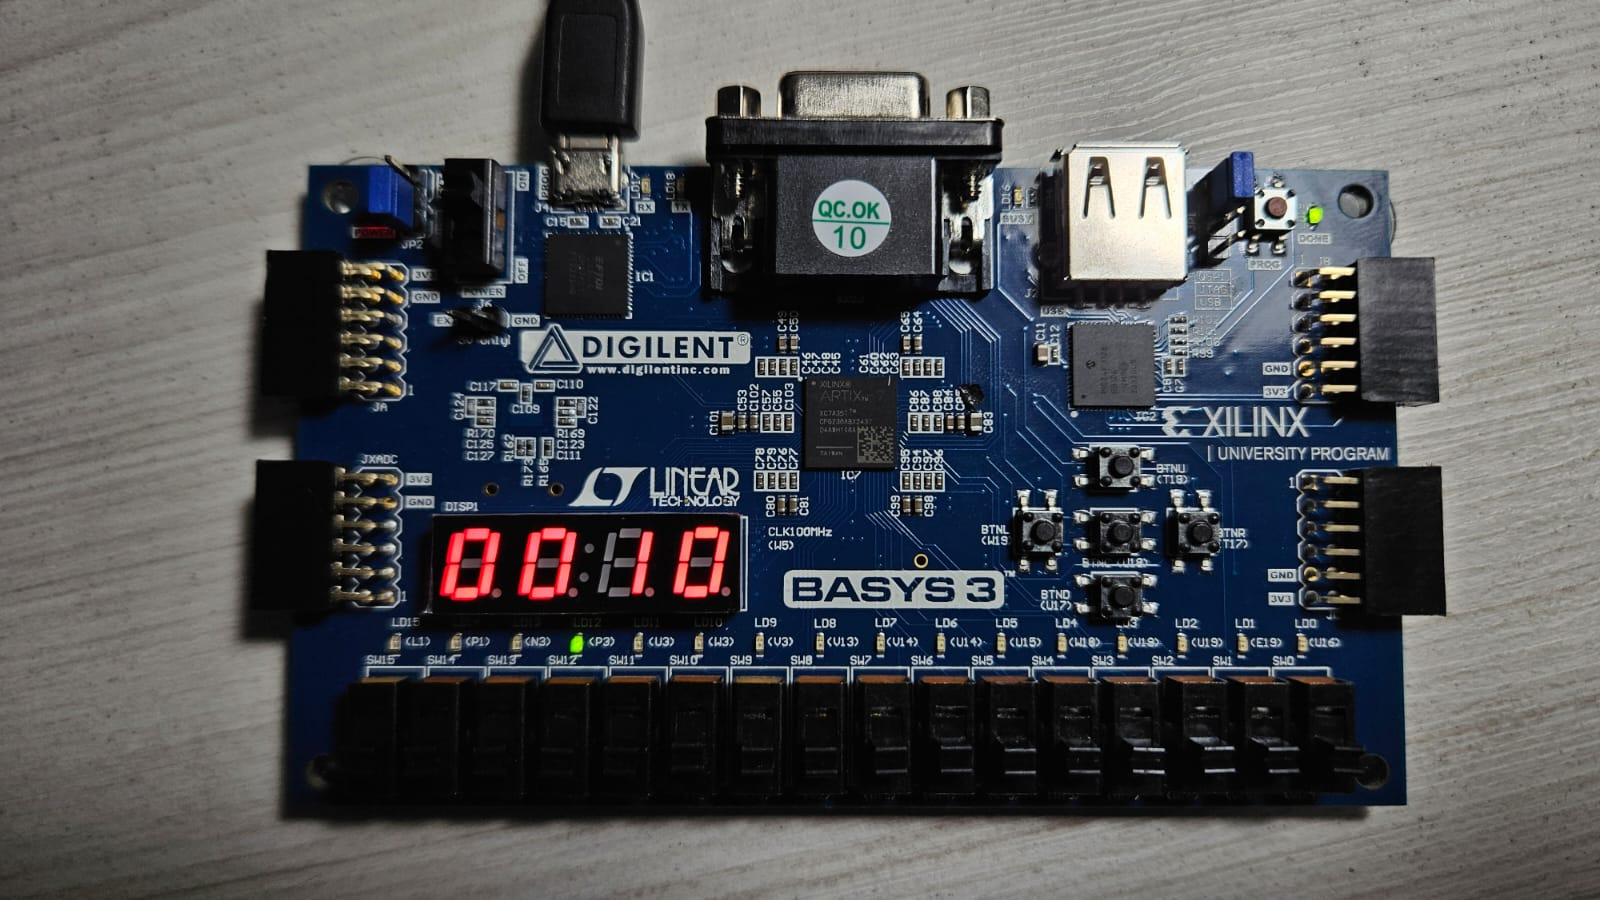
\includegraphics[width=0.6\textwidth]{img/fpga6.png}
    \caption{Prueba con $B=0$.}
    \label{fig:fpga6}
\end{figure}

\begin{figure}[H]
    \centering
    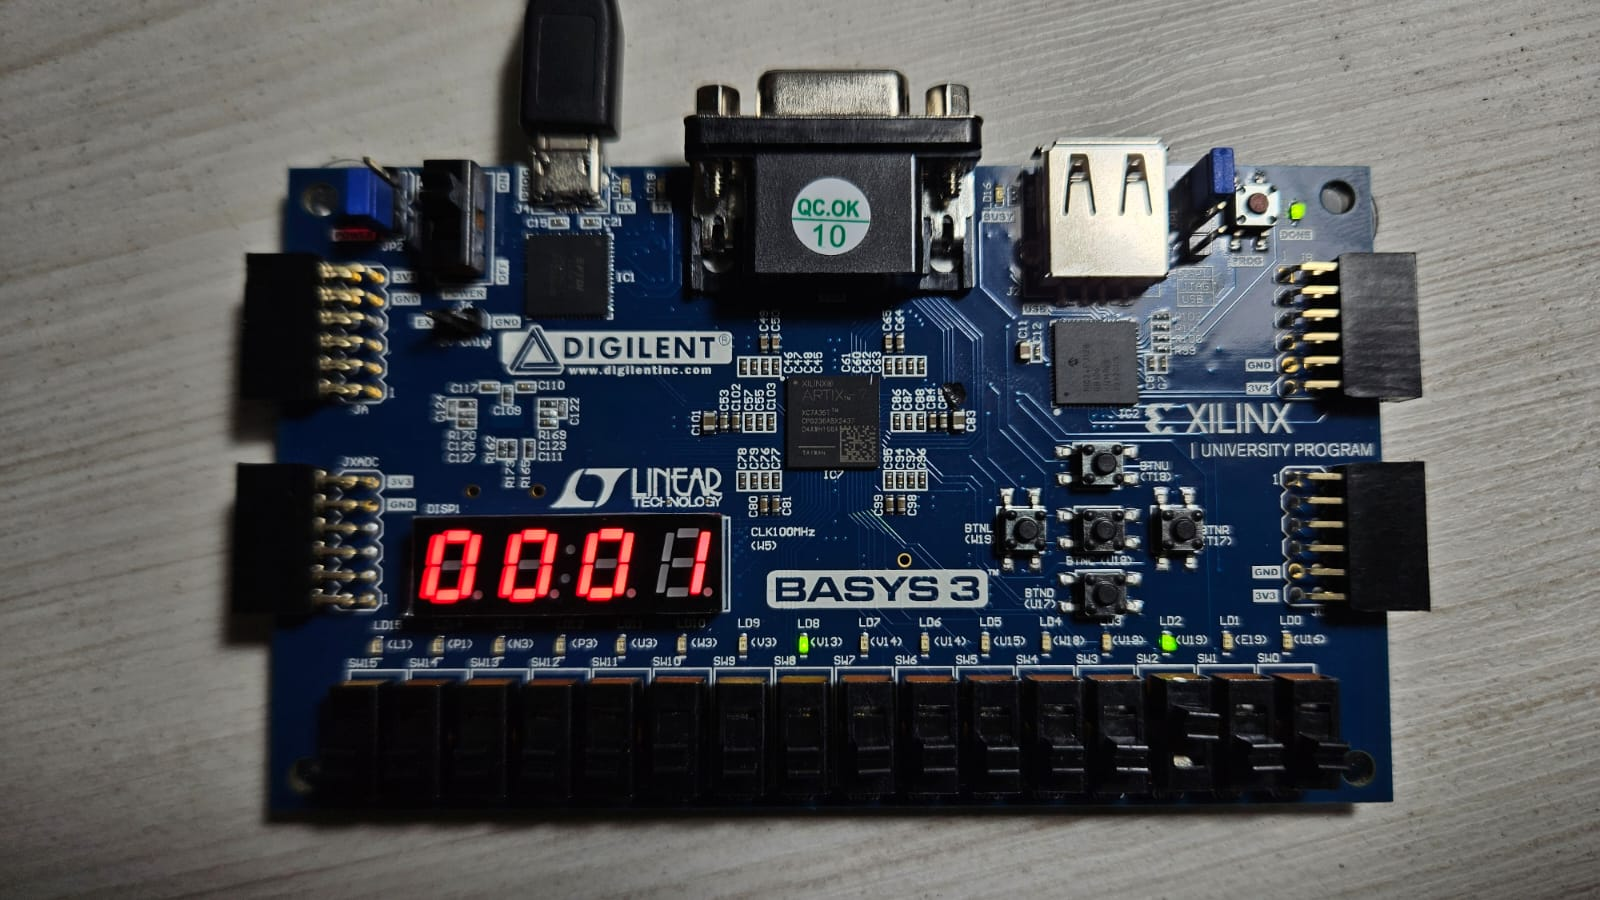
\includegraphics[width=0.6\textwidth]{img/fpga7.png}
    \caption{Prueba con $B=100$.}
    \label{fig:fpga7}
\end{figure}

\begin{figure}[H]
    \centering
    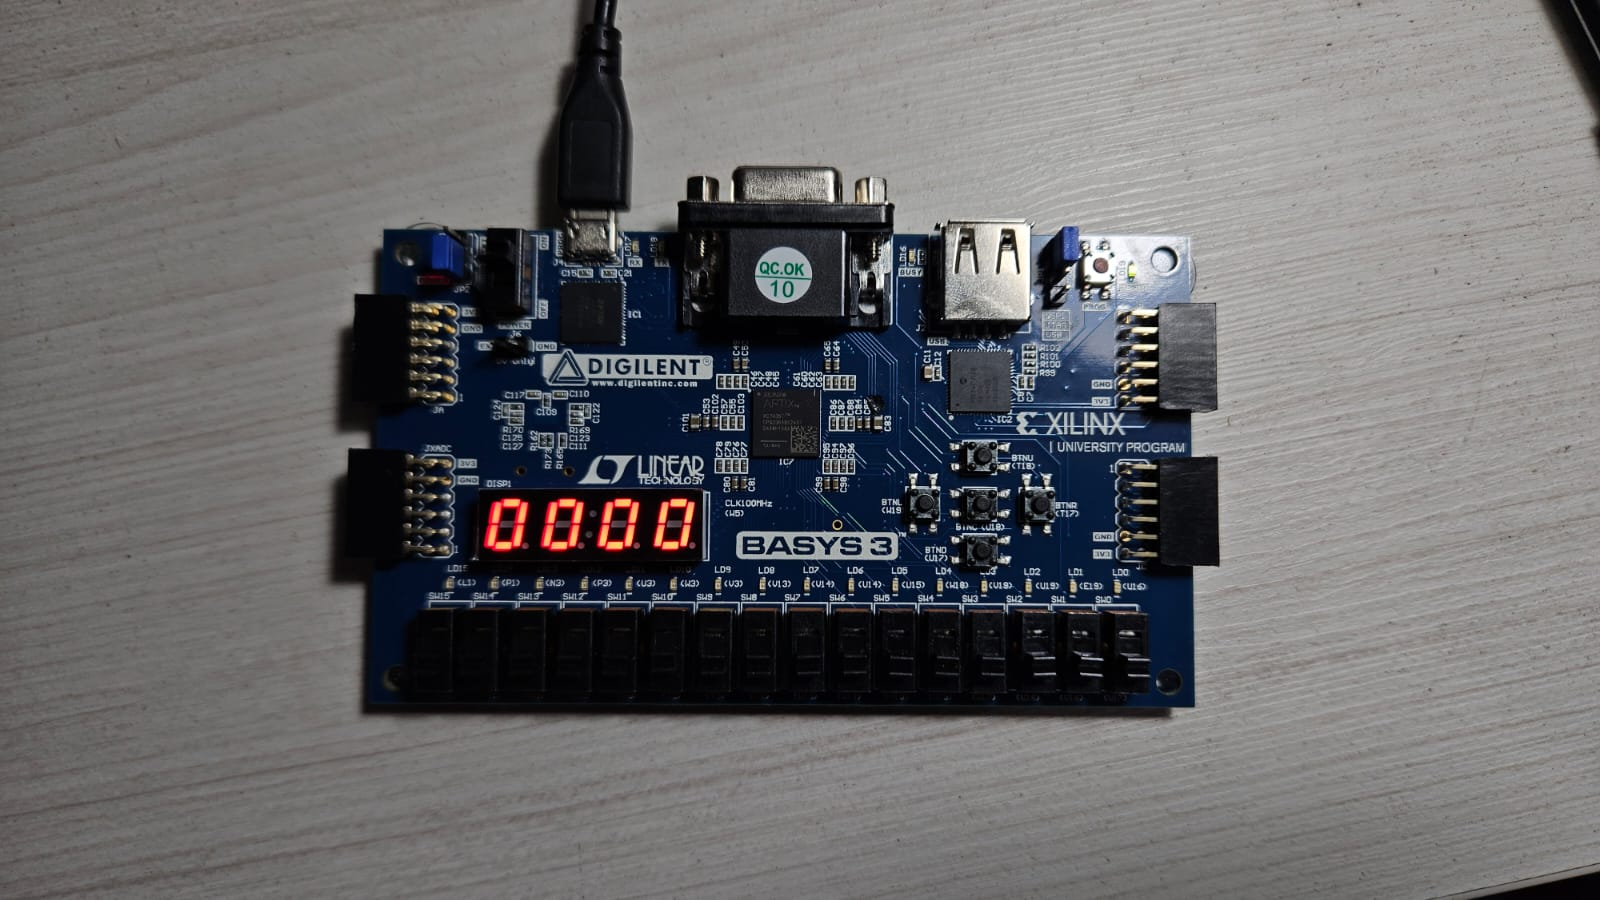
\includegraphics[width=0.6\textwidth]{img/fpga8.png}
    \caption{FPGA despues del reset}
    \label{fig:fpga8}
\end{figure}
